\documentclass{simple}

\title[Common Bullshit]{Common Bullshit: Când oamenii mănâncă \ldots{} rahat}
\institute{}
\author[Răzvan Deaconescu]{Răzvan Deaconescu \\
razvan.deaconescu@cs.pub.ro}
\date{26 aprilie 2018}

\begin{document}

\frame{\titlepage}

\begin{frame}{Common Bullshit}
  \centering
  \Large
  \pause vorbe des întâlnite \\
  \pause luate pe de-a gata \\
  \pause considerate aproape mereu valabile/adevărate \\
  \pause netrecute printr-un filtru critic \\
\end{frame}

\begin{frame}{Cadru de prezentare/discuție}
  \pause X is bullshit
  \begin{itemize}
    \pause \item nu înseamnă că X e fals, de multe ori e adevărat
    \pause \item dar \ldots
      \begin{itemize}
        \pause \item X e văzut ca valabil adevărat aproape mereu și aproape peste tot, indiferent de circumstanțe
        \pause \item X e văzut ca adevăr absolut, fără nuanțe
        \pause \item X e văzut exagerat
        \pause \item X e preocupat despre ideal, cum e bine să fie, nu despre cum e de fapt
      \end{itemize}
    \pause \item apariția X are o cauză: există o problemă, o situație urâtă, neplăcută pe care vrem să o corectăm
      \begin{itemize}
        \pause \item X este o soluție, dar \ldots
        \pause \item soluția urmărește intenția, nu rezultatul
      \end{itemize}
  \end{itemize}
\end{frame}

\begin{frame}{Intenție și rezultat}
  \centering
  \pause \textit{One of the great mistakes is to judge policies and programs by their intentions rather than their results.}\\
  \vspace{3mm}
  \hfill \textit{Milton Friedman} \\
  \vspace{2cm}
  \centering
  \pause \textit{When idealism meets reality, it's rarely reality that backs down.} \\
  \vspace{3mm}
  \hfill \textit{Michael Liberty (Starcraft)}
\end{frame}

\begin{frame}{Comunismul funcționează}
  \centering
  \begin{figure}
    
\includegraphics[width=0.7\textwidth]{img/communism}
  \end{figure}
  \tiny
  \url{https://en.wikipedia.org/wiki/Communism}
\end{frame}

\begin{frame}{Omul face haina, nu haina pe om}
  \begin{itemize}
    \pause \item cauză: prea mult marketing și superficialitate
    \pause \item soluția: contează ce ai înăuntru, it's the inside that counts, don't judge a book by its cover
    \pause \item dar \ldots
      \begin{itemize}
        \pause \item oamenii își formează părerea după aspect, prima impresie contează
        \pause \item modul în care te prezinți și arăți influențează ce spui, ce faci, limbajul non-verbal
        \pause \item aspectul, hainele, stilul spun dacă ești: preocupat, atent, îngrijit, curat
        \pause \item aspectul e parte din tine, nu-l poți separa, spune ceva despre tine (nu tot)
      \end{itemize}
  \end{itemize}
\end{frame}

\begin{frame}{Oamenii se schimbă}
  \begin{itemize}
    \pause \item cauză: oamenii au defecte care se pot corecta, speranța în bine, în perfectibil
    \pause \item soluția: oamenii se schimbă
    \pause \item dar \ldots
      \begin{itemize}
        \pause \item oamenii se schimbă doar dacă vor sau dacă sunt supuși unor presiuni enorme sau traume
        \pause \item așteptarea că oamenii se schimbă (by default) nu e realistă
        \pause \item by default oamenii nu se schimbă, dar avem speranța că se pot schimba
        \pause \item reputația se bazează pe trecut, pe ce ai făcut, instinctiv știm că va fi cum a fost
        \pause \item ține foarte mult de om
      \end{itemize}
  \end{itemize}
\end{frame}

\begin{frame}{Good things happen to good people}
  \begin{itemize}
    \pause \item cauză: nevoie/instinct de altruism, reciprocitate
    \pause \item soluția: good things happen to good people
    \pause \item dar \ldots
      \begin{itemize}
        \pause \item uneori lucrurile bune nu aduc o schimbare din partea celorlalți
        \pause \item așteptarea că oamenii sunt (by default) reciproci nu e realistă
        \pause \item by default oamenii nu sunt reciproci, dar avem speranța că vor fi reciproci
        \pause \item ține foarte mult de om
      \end{itemize}
  \end{itemize}
\end{frame}

\begin{frame}{Oamenii sunt egali}
  \begin{itemize}
    \pause \item cauză: abuzuri ale unor oameni, nedreptăți
    \pause \item soluția: oamenii sunt egali
    \pause \item dar \ldots
      \begin{itemize}
        \pause \item oamenii nu sunt egali biologic/genetic, fizic, intelectual
        \pause \item oamenii nu au același potențial
        \pause \item oamenii nu au aceleași preferințe
        \pause \item oamenii nu au aceleași șanse
        \pause \item oamenii evoluează sau stagnează
      \end{itemize}
    \pause \item putem vorbi de drepturi egale, tratament egal în fața legii
    \pause \item Tudor Arghezi: \textit{Slova de foc și slova făurită}
    \pause \item Vegeta vs Goku: \textit{However, you were born with a natural talent far above that of my own. No amount of training could have closed the gap between us.}
  \end{itemize}
\end{frame}

\begin{frame}{Oamenii sunt egali: fizic}
  \centering
  \begin{figure}
    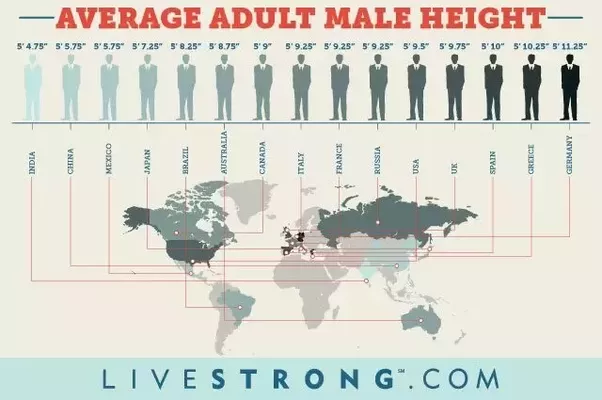
\includegraphics[width=0.9\textwidth]{img/male-height}
  \end{figure}
\end{frame}

\begin{frame}{Bărbații și femeile sunt la fel}
  \begin{itemize}
    \pause \item cauză: abuzuri ale bărbaților, discriminare, lipsă de drepturi femei
    \pause \item soluția: bărbații și femeile sunt la fel
    \pause \item dar \ldots
      \begin{itemize}
        \pause \item bărbații și femeile sunt biologic/fizic diferiți
        \pause \item bărbații și femeile sunt endocrinologic diferiți
        \pause \item bărbații și femeile sunt psihologic diferiți
        \pause \item bărbații și femeile au strategii sexuale diferite și comportament sexual diferit
      \end{itemize}
    \pause \item la fel, putem vorbi de drepturi egale, tratament egal în fața legii
    \pause \item există condiționări sociale care pot fi corectate și condiționări biologice (firmware biologic) care sunt acolo mereu
  \end{itemize}
\end{frame}

\begin{frame}{Bărbații și femeile sunt la fel: hormoni}
  \pause testosteron \\
  \begin{itemize}
    \pause \item femei: 6-86 ng/dl
    \pause \item bărbați: 270-1100 ng/dl
  \end{itemize}
  \pause estrogen \\
  \begin{itemize}
    \pause \item femei: 15-350 pg/ml
    \pause \item bărbați: 10-40 pg/ml
  \end{itemize}
\end{frame}

\begin{frame}{Bărbații și femeile sunt la fel: fizic}
  \centering
  \begin{figure}
    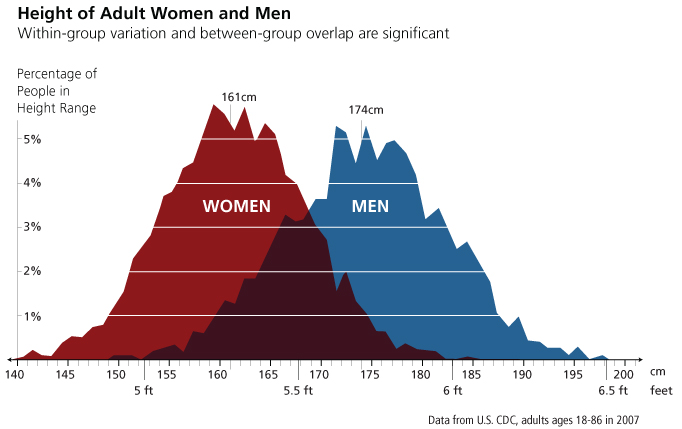
\includegraphics[width=0.8\textwidth]{img/male-female-height}
  \end{figure}
\end{frame}

\begin{frame}{Bărbații și femeile sunt la fel: fizic (2)}
  \centering
  \begin{figure}
    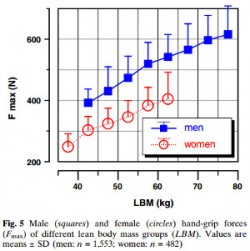
\includegraphics[width=0.5\textwidth]{img/male-female-grip}
  \end{figure}
\end{frame}

\begin{frame}{Bărbații și femeile sunt la fel: fizic (3)}
  \centering
  \begin{figure}
    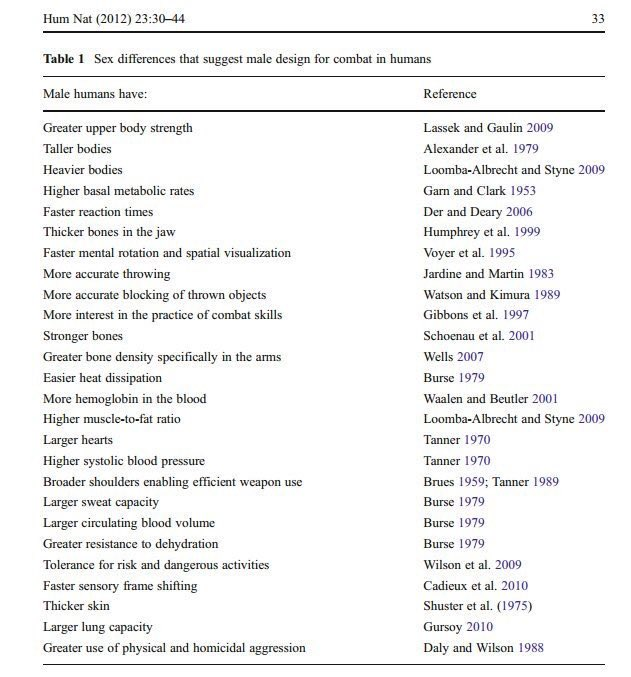
\includegraphics[width=0.7\textwidth]{img/male-combat}
  \end{figure}
\end{frame}

\begin{frame}{Bărbații și femeile sunt la fel: IQ}
  \centering
  \begin{figure}
    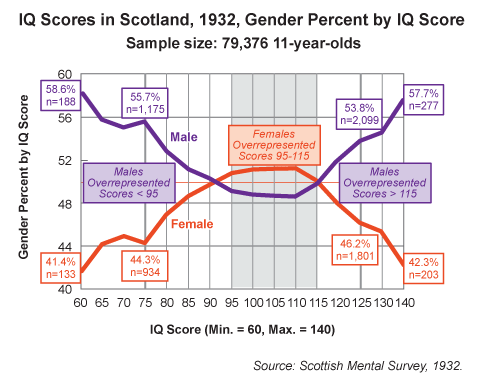
\includegraphics[width=0.7\textwidth]{img/male-female-iq}
  \end{figure}
\end{frame}

\begin{frame}{Bărbații și femeile sunt la fel: activități}
  \centering
  \begin{figure}
    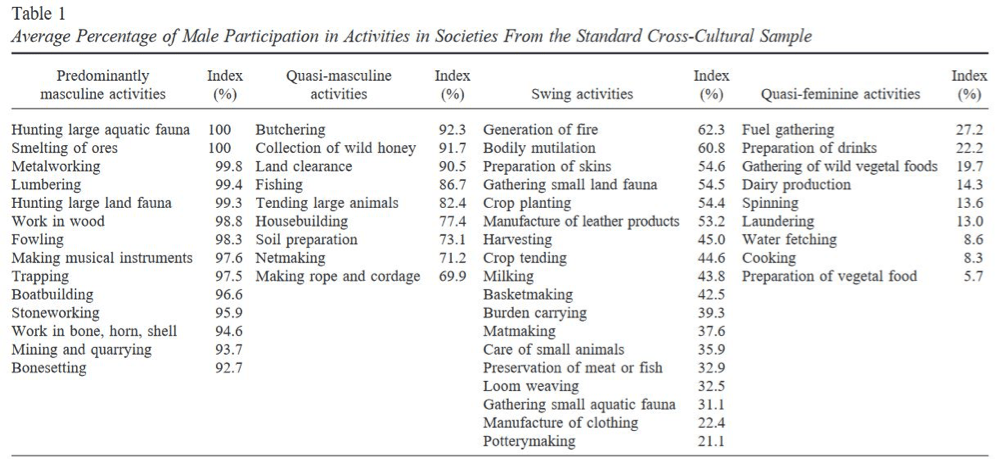
\includegraphics[width=\textwidth]{img/male-activities}
  \end{figure}
\end{frame}

\begin{frame}{All you need is love}
  \begin{itemize}
    \pause \item cauză: nevoie de cineva lângă tine, dragoste necondiționată, nevoie sexuală
    \pause \item soluția: dragoste e ceea ce contează
    \pause \item dar \ldots
      \begin{itemize}
        \pause \item nu există nimic necondiționat, e un proces
        \pause \item \textit{Nobody gets a soul mate. It don't happen. All you gonna get in life if you lucky is a mate.} (Chris Rock)
        \pause \item oamenii trăiesc pentru multe lucruri: dragostea/partenerul nu e totul
      \end{itemize}
  \end{itemize}
\end{frame}

\begin{frame}{Reach for the stars}
  \begin{itemize}
    \pause \item cauză: oameni demotivați, abuzați de părinți, rude, obligați să facă lucruri de rutină
    \pause \item soluția: reach for the stars
    \pause \item dar \ldots
      \begin{itemize}
        \pause \item \textit{Per aspera ad astra.}
        \pause \item nu toți oamenii pot
        \pause \item nu toți oamenii vor
        \pause \item nu toți oamenii au șanse
        \pause \item life's a bitch
      \end{itemize}
  \end{itemize}
\end{frame}

\begin{frame}{Communication is key}
  \begin{itemize}
    \pause \item cauză: neînțelegeri, frustrări, temeri ale oamenilor
    \pause \item soluția: să comunicăm să fie bine
    \pause \item dar \ldots
      \begin{itemize}
        \pause \item multe întâlniri sunt pierdere de timp
        \pause \item la mai mult de N persoane (YMMV) iese circle jerk (agile, anyone?)
        \pause \item în intimitate, comunicarea faptică e moartea pasiunii
        \pause \item comunicarea/faptele omoară emoția/tensiunea
      \end{itemize}
  \end{itemize}
\end{frame}

\begin{frame}{Să fie pace}
  \textit{Imagine all the people living life in peace.} (John Lennon) \\
  \begin{itemize}
    \pause \item cauză: violență, războaie, suferință
    \pause \item soluția: să fie pace
    \pause \item dar \ldots
      \begin{itemize}
        \pause \item oamenii (mai ales bărbații) au tendințe agresive
        \pause \item se acumulează inerent frustrări personale, sociale, naționale, care caută o eliberare
        \pause \item conflictul a dus la progres tehnologic
        \pause \item \textit{Si vis pacem, para bellum.}
      \end{itemize}
  \end{itemize}
\end{frame}

\begin{frame}{Sumar}
  \pause X is bullshit
  \begin{itemize}
    \pause \item există o problemă Y pe care X vrea să o rezolve
    \pause \item nu există panaceu
    \pause \item X nu se aplică peste tot, uneori nu merge deloc, alteori în anumite situații
    \pause \item X nu e adevărat mereu așa cum se zice (\textit{read the fine print})
  \end{itemize}
  \pause intenții/ideal vs rezultate/realitate
\end{frame}

\begin{frame}{De ce să-mi bat capul?}
  \pause \textbf{I want to live in unicorn land!}\\
  \vspace{1cm}
  \pause Unicorn land nu e rău, dar \ldots
  \begin{itemize}
    \pause \item vrei să știi, vrei să înțelegi lucrurile
    \pause \item vrei să faci ceva cu alți oameni, să schimbi, să îmbunătățești
    \pause \item vrei să nu fii dezamăgit, sau când ești, să știi de ce s-a întâmplat
    \pause \item \textit{shit happens}, nu ești în control
  \end{itemize}
\end{frame}

\begin{frame}{Ce pot să fac?}
  \centering
  \Large
  \pause Stop. Look. Listen. \\
  \pause daydream, meditează, rumegă \\
  \pause debate, dissent, challenge \\
\end{frame}

\begin{frame}{În final}
  \pause \textit{Dave Rubin: You were a Marxist at one time in your life.} \\
  \pause \textit{Thomas Sowell: But it's not that unusual.} \\
  \pause \textit{Dave Rubin: What was your wakeup to what was wrong with that line of thinking?} \\
  \pause \textit{Thomas Sowell: Facts.} \\
\end{frame}

\end{document}
